\documentclass{article}
\usepackage{helvet}
\renewcommand{\familydefault}{\sfdefault}
\usepackage{listings}
\usepackage{wrapfig}
\usepackage{graphicx}
\graphicspath{ {/} }
\title{Heuristic Analysis for Isolation Game}
\author{John Carpenter}
\begin{document}
\maketitle{}
\section{Isolation Analysis}
For this isolation game, a game agent was built that was able to defeat a variety of different computer opponents roughly
85\% time. The game agent used a combination of minimax and alphabeta pruning to search through
the game space for the correct moves.

\subsection{Discussion}
\textbf{Performance}\newline
After running the tournament a number of times one of the important factors in the outcome was the depth of search that
the program was able to complete. Turns must be completed in 150ms or the game was forfeited with a loss. To this end the performance of the \verb|get_move| determined how often the program was able to win. Optimizing this method was important to a successful run.
While there wasn't any global metrics collected a cursory calculation showed that the number of searches that went to full-depth was less than 40\% and those were likely near the end of the match only\newline

In creating the game agent we implemented a tree-node architecture with the \verb|GameNode.py| class. That architecture allowed
for flexible tree configurations and separated the construction of the tree with it's scoring/pruning functions. However, considering the unittest were written first we had to modify some of the
code to function within the parameters and it lost some of its effectiveness.\newline

It would be worthwhile to continue some optimization on the \verb|get_move| in order to see it's impact on the solution.
The first step might be collecting better metrics on the performance of the search and scoring routines and profiling the method calls in more depth.


\subsection{Heuristics}
In order to evaluate the board state at each we created 4 heuristics as a measure of the quality of the board. The
goal of this section was to arrive at a heuristic that was able to statistically outperform the \texttt{\detokenize{ID_Improved}}
model that was provided.\newline

\begin{itemize}
  \item Heuristic 1 - Baseline Low Performance
  \item Heuristic 2 - Moves Left (\texttt{\detokenize{ID_Improved}} model)
  \item Heuristic 3 - Warnsdorf's rules
  \item Heuristic 4 - Modified Moves Left
\end{itemize}

\textbf{Notes:} The results and analysis here are based upon a limited run of a couple hundred game instances. As shown in the sections below
there is a large variation in the winning percentages. Given the variability and small sample size the results may not be statistically significant


The details of each of the repective measures are in their sections below.
\subsubsection{Heuristic 1 - Baseline Low Performance}

The first heuristic was done to provide a baseline for the remaining test cases. This should allow us to
understand how much a change in the scoring heuristic is expected to impact the testing performance.\newline

\textbf{Results}\newline
As expected, the results from the first heuristic performed worse than the \texttt{\detokenize{ID_Improved}} model.

\begin{verbatim}
  *************************
   Evaluating: ID_Improved
  *************************

  Playing Matches:
  ----------
    Match 1: ID_Improved vs   Random    	Result: 19 to 1
    Match 2: ID_Improved vs   MM_Null   	Result: 18 to 2
    Match 3: ID_Improved vs   MM_Open   	Result: 13 to 7
    Match 4: ID_Improved vs MM_Improved   Result: 17 to 3
    Match 5: ID_Improved vs   AB_Null     Result: 18 to 2
    Match 6: ID_Improved vs   AB_Open   	Result: 18 to 2
    Match 7: ID_Improved vs AB_Improved 	Result: 17 to 3

  Results:
  ----------
  ID_Improved         85.71%

  *************************
     Evaluating: Student
  *************************

  Playing Matches:
  ----------
    Match 1:   Student   vs   Random    	Result: 17 to 3
    Match 2:   Student   vs   MM_Null   	Result: 16 to 4
    Match 3:   Student   vs   MM_Open   	Result: 13 to 7
    Match 4:   Student   vs MM_Improved 	Result: 13 to 7
    Match 5:   Student   vs   AB_Null   	Result: 17 to 3
    Match 6:   Student   vs   AB_Open   	Result: 13 to 7
    Match 7:   Student   vs AB_Improved 	Result: 10 to 10

  Results:
  ----------
  Student             70.71%
\end{verbatim}

\subsubsection{Heuristic 2}

The second heuristic was identical to the \texttt{\detokenize{ID_Improved}} model. We ran this model to demonstrate
some of the variability in the win \%. Even within the tests in this document we see the range of win \% from the \texttt{\detokenize{ID_Improved}}
vary between 82\% and 90\%.\newline
\textbf{Results}\newline
\begin{verbatim}
  *************************
   Evaluating: ID_Improved
  *************************

  Playing Matches:
  ----------
    Match 1: ID_Improved vs   Random    	Result: 20 to 0
    Match 2: ID_Improved vs   MM_Null   	Result: 20 to 0
    Match 3: ID_Improved vs   MM_Open   	Result: 17 to 3
    Match 4: ID_Improved vs MM_Improved 	Result: 15 to 5
    Match 5: ID_Improved vs   AB_Null   	Result: 20 to 0
    Match 6: ID_Improved vs   AB_Open   	Result: 16 to 4
    Match 7: ID_Improved vs AB_Improved 	Result: 15 to 5


  Results:
  ----------
  ID_Improved         87.86%

  *************************
     Evaluating: Student
  *************************

  Playing Matches:
  ----------
    Match 1:   Student   vs   Random    	Result: 19 to 1
    Match 2:   Student   vs   MM_Null   	Result: 20 to 0
    Match 3:   Student   vs   MM_Open   	Result: 18 to 2
    Match 4:   Student   vs MM_Improved 	Result: 17 to 3
    Match 5:   Student   vs   AB_Null   	Result: 19 to 1
    Match 6:   Student   vs   AB_Open   	Result: 18 to 2
    Match 7:   Student   vs AB_Improved 	Result: 17 to 3


  Results:
  ----------
  Student             91.43%
\end{verbatim}

\subsubsection{Heuristic 3}

\begin{wrapfigure}{r}{0.4\textwidth}
    \centering
    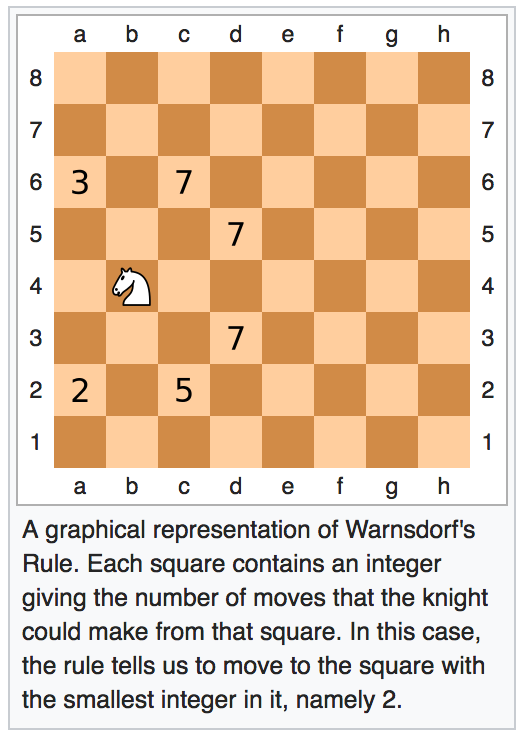
\includegraphics[width=0.4\textwidth]{chessboard}
\end{wrapfigure}

The third heuristic attempted to utilize a slightly different approach to scoring the model. \newline
There is a mathematical problem, called the Knights Tour that is relevant to this game. In this problem the goal
is to move a Knight around a chessboard such that you touch every point on the board without visiting the same point twice.
In this problem, the mathematician H.C Warnsdorf determined that the solution involves always moving to the point with the fewest number of connected locations. It is called
 Warnsdorf's rule.\newline
 In order to implement a variant of that form, we want the program to choose a location with the minimum number of moves (greater than 0),
 and the opponent to choose the move with the most amount of moves. (Although the second part isn't as crucial to the formula). We based
 the quality of the board as:\newline

 \begin{lstlisting}[language = python]
   if(player_moves_left >= 2):
       return 8 - float(player_moves_left)
   else:
       return -1
 \end{lstlisting}

See: \url{\detokenize{https://en.wikipedia.org/wiki/Knight's_tour#Warnsdorf.27s_rule}}\newline


\textbf{Results}\newline
Using the Warnsdorf heuristic proved to have a negative effect on the winning percentage. In the case below,
the Warnsdorf won 80.7\% to the \texttt{\detokenize{ID_Improved}} at 91\%. I suspect the reason behind this
is that nearing the end of the game, the opponent will have taken the larger numbers near the center and forced
the player to the corners. Since Warnsdorf's rule might require the larger numbers near the end of the game to
allow it to work.

\begin{verbatim}
  *************************
   Evaluating: ID_Improved
  *************************

  Playing Matches:
  ----------
    Match 1: ID_Improved vs   Random    	Result: 20 to 0
    Match 2: ID_Improved vs   MM_Null   	Result: 20 to 0
    Match 3: ID_Improved vs   MM_Open   	Result: 17 to 3
    Match 4: ID_Improved vs MM_Improved 	Result: 19 to 1
    Match 5: ID_Improved vs   AB_Null   	Result: 17 to 3
    Match 6: ID_Improved vs   AB_Open   	Result: 19 to 1
    Match 7: ID_Improved vs AB_Improved 	Result: 16 to 4


  Results:
  ----------
  ID_Improved         91.43%

  *************************
     Evaluating: Student
  *************************

  Playing Matches:
  ----------
    Match 1:   Student   vs   Random    	Result: 18 to 2
    Match 2:   Student   vs   MM_Null   	Result: 19 to 1
    Match 3:   Student   vs   MM_Open   	Result: 14 to 6
    Match 4:   Student   vs MM_Improved 	Result: 14 to 6
    Match 5:   Student   vs   AB_Null   	Result: 20 to 0
    Match 6:   Student   vs   AB_Open   	Result: 14 to 6
    Match 7:   Student   vs AB_Improved 	Result: 14 to 6


  Results:
  ----------
  Student             80.71%
\end{verbatim}

\subsubsection{Heuristic 4}

The final heuristic measure is a variant on the \texttt{\detokenize{ID_Improved}} model. In this model we weight the opponents
remaining moves as more important in the calculation to by doubling its effect. This has the effect of trying to minimize
the opponents available moves while not being as concerned about the programs number of moves. \newline

\begin{lstlisting}[language = python]
  return float(player_moves_left) - 2*float(opponent_moves_left)
\end{lstlisting}
\newline
\textbf{Results}\newline
This heuristic model is the first of the collection that seems to consistently perform better than the default \texttt{\detokenize{ID_Improved}} model.
The model typically averaged 5-6\% higher win percentage although that is still within the statistical variance we have seen in the tests.

\begin{verbatim}
  *************************
   Evaluating: ID_Improved
  *************************

  Playing Matches:
  ----------
    Match 1: ID_Improved vs   Random    	Result: 17 to 3
    Match 2: ID_Improved vs   MM_Null   	Result: 19 to 1
    Match 3: ID_Improved vs   MM_Open   	Result: 16 to 4
    Match 4: ID_Improved vs MM_Improved 	Result: 13 to 7
    Match 5: ID_Improved vs   AB_Null   	Result: 19 to 1
    Match 6: ID_Improved vs   AB_Open   	Result: 16 to 4
    Match 7: ID_Improved vs AB_Improved 	Result: 16 to 4


  Results:
  ----------
  ID_Improved         82.86%

  *************************
     Evaluating: Student
  *************************

  Playing Matches:
  ----------
    Match 1:   Student   vs   Random    	Result: 16 to 4
    Match 2:   Student   vs   MM_Null   	Result: 18 to 2
    Match 3:   Student   vs   MM_Open   	Result: 16 to 4
    Match 4:   Student   vs MM_Improved 	Result: 18 to 2
    Match 5:   Student   vs   AB_Null   	Result: 20 to 0
    Match 6:   Student   vs   AB_Open   	Result: 17 to 3
    Match 7:   Student   vs AB_Improved 	Result: 17 to 3


  Results:
  ----------
  Student             87.14%
\end{verbatim}

\subsection{Recommendations}

The evaluation function in the \texttt{\detokenize{ID_Improved}} model provides a very strong opponent and does so efficiently with a minimum amount of processing required. The improvements on the model will be minimal but can be improved by reducing some of the dependence on the players position.\newline

\textbf{Suggested Evaluation Model}\newline

\begin{lstlisting}[language = python]
  return float(player_moves_left) - 2*float(opponent_moves_left)
\end{lstlisting}

From Warnsdorf's rule, we know that the optimal route for a single player within the game is to choose the route with the fewest number of connecting nodes. However, within a competitive gameplay this does not always ensure a winning scenario. In fact, quite the opposite. Nearing the end of the game the player needs to optimize their moves remaining, while minimizing the opponents. The latter being much more important. The evaluation model we have chosen seeks to minimize the opponents movements as much as possible. Slightly more agressive than the \texttt{\detokenize{ID_Improved}} it tries to win the game without worrying too much about the players position.

\begin{enumerate}
\item For a single player the optimal move is to node with the fewest connections, therefore the number of player moves the player can reach at each node is relatively independent of its strength.

\item Nearing the end game, the player should try to force the opponent into a trapped position. This can be done by eliminating the available moves by the opponent. The second term in the calculation \verb|(- 2*float(opponent_moves_left))| accounts for this.

\item Even though the players movement is relatively independent from number of connecting nodes, during the final moves of the game the player needs to continue to move to positions that have connecting nodes. That is why the first term in the parameter (\verb|float(player_moves_left)|) is left in.
\end{enumerate}


\subsection{Future Work}

The game playing agent was successful in competing in the simulated tournament against
a small variety of simple opponents. However competing against a stronger opponent such as
the \texttt{\detokenize{ID_Improved}} model the results are not as conclusive. Here are
some recommendations that would improve the strength of the game agent model.\newline
\begin{enumerate}
\item Improve the speed of the \verb|get_move| function. The speed of this function determines
the depth to which the algorithm can search. Through a combination of method profiling and optimizations
the function will be able to search deeper into the game producing a more certain outcome.

\item Following the improvement in speed, parallel processing and threading will allow the search to
execute on multiple processors simultaneously. This will improve the depth at which searches can operate.

\item Improved Heuristics. The 4th heuristic that puts a higher weight on the opponents position versus the
players position showed to have a marginal increase in winning percentage.

\item Better Metrics and Analysis. In order to measure the increase from the previous two items, we need an
accurate, statistically valid baseline. We will also need better visibility into the algorithms performance
and the impact any changes have on the outcome. Metrics such as the \% of searches going to full-depth, and the
average depth at timeout would go a long way in determining which changes are beneficial for the algorithm.
\end{enumerate}




\end{document}
